\subsection{Modello architetturale}
Il \textit{sistema}\textsubscript{\textit{G}} richiede la capacità di elaborare dati provenienti da diverse fonti in tempo reale e di fornire una visualizzazione immediata e continua di tali dati, permettendo di monitorarne gli andamenti e di rilevare eventuali anomalie. 
Per tale scopo, l'\textit{architettura}\textsubscript{\textit{G}} di \textit{sistema}\textsubscript{\textit{G}} adottata è la \textit{$\kappa$-architecture}.

\subsubsection{$\kappa$-architecture}
L'\textit{architettura}\textsubscript{\textit{G}} Kappa è un modello di elaborazione dati in streaming che offre un'alternativa all'\textit{architettura}\textsubscript{\textit{G}} Lambda. Il suo obiettivo principale è unificare lo \textit{stream processing} e il \textit{batch processing} all'interno di un unico \textit{stack tecnologico}\textsubscript{\textit{G}}, mantenendo il \textit{sistema}\textsubscript{\textit{G}} in real time.

\paragraph{Vantaggi}
\begin{itemize}
    \item Semplice da implementare e gestire, costi di manutenzione ridotti;
    \item Assicura coerenza tra l'analisi in tempo reale e batch.
\end{itemize}

\paragraph{Svantaggi}
\begin{itemize}
    \item Potenziale rallentamento dell'analisi in tempo reale, meno flessibile rispetto a Lambda.
\end{itemize}

\subsubsection{Componenti di sistema}
\begin{figure}[H]
    \centering
    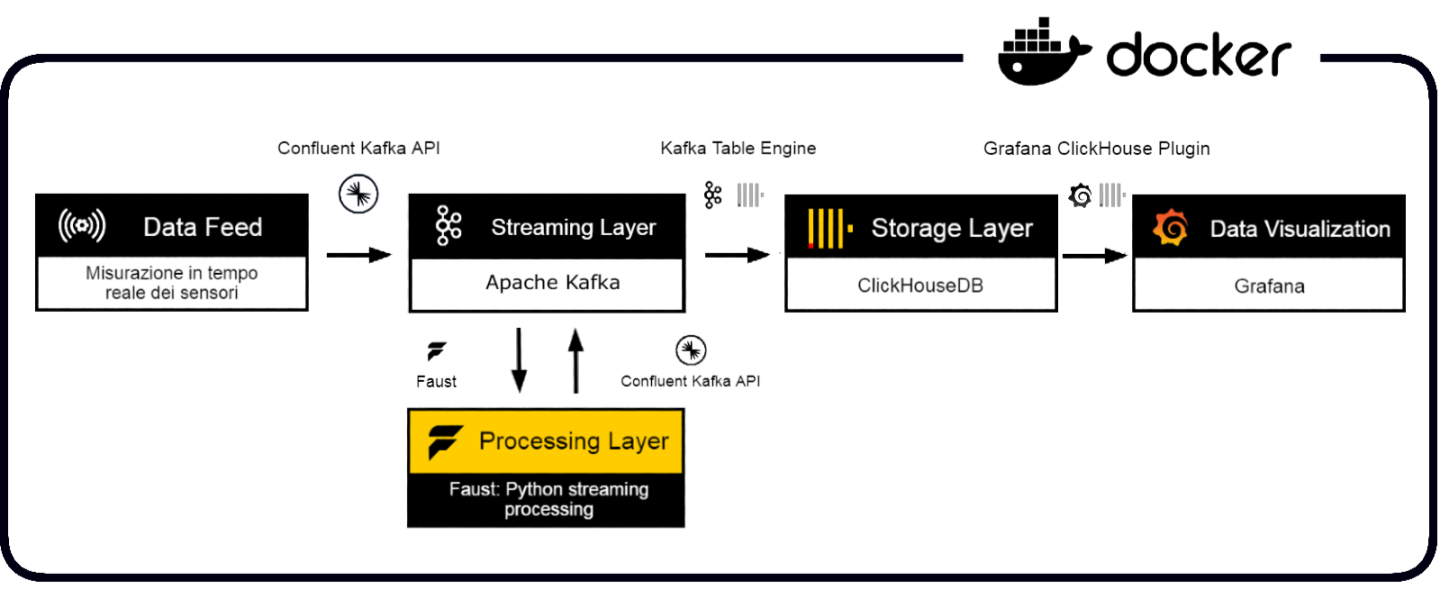
\includegraphics[width=1\textwidth]{../Images/SpecificaTecnica/Architettura_PB_microservices2.png}
    \caption{Componenti dell'architettura - InnovaCity}
    \label{fig: componenti_architettura}
\end{figure}

\begin{itemize}
    \item \textbf{Data source:} Le sorgenti dati sono costituite da simulatori di sensori IoT dislocati sul territorio cittadino. Questi sensori sono in grado di inviare, ad intervalli regolari, messaggi contenenti misurazioni allo streaming layer;
    
    \item \textbf{Streaming layer:} Lo streaming layer gestisce i dati in arrivo in tempo reale, per poi archiviarli sistematicamente nello \textit{storage}\textsubscript{\textit{G}} layer;
    
    Lo streaming layer è composto da:
    \begin{itemize}
        \item \textbf{Apache Kafka:} \textit{Kafka}\textsubscript{\textit{G}}\textsubscript{\textit{G}} è un \textit{sistema}\textsubscript{\textit{G}} di messaggistica distribuito che consente di pubblicare, sottoscrivere e archiviare messaggi in tempo reale. \textit{Kafka}\textsubscript{\textit{G}}\textsubscript{\textit{G}} è utilizzato per ricevere i dati dai sensori e renderli disponibili per l'elaborazione in tempo reale e batch;
        
        \item \textbf{Zookeeper:} Per il coordinamento e la gestione dei cluster \textit{Kafka}\textsubscript{\textit{G}};
        \item \textbf{Schema Registry:} Definizione e gestione degli schemi per i dati in streaming.
    \end{itemize}

    \item \textbf{Processing layer:} Il processing layer è costituito da Faust che consuma i dati dallo streaming layer e li processa in tempo reale. Faust è una libreria \textit{Python}\textsubscript{\textit{G}} che permette l'elaborazione di \textit{stream}\textsubscript{\textit{G}} di dati in tempo reale. Faust è utilizzato per elaborare i dati in arrivo tramite un modello per il calcolo del punteggio di salute che poi viene reso nuovamente disponibili allo streaming layer;
    
    \item \textbf{Storage layer:} Lo \textit{storage}\textsubscript{\textit{G}} layer è costituito da un \textit{database}\textsubscript{\textit{G}} column-oriented, \textit{ClickHouse}\textsubscript{\textit{G}}, che archivia i dati in arrivo dallo streaming layer. Questi dati sono disponibili per l'analisi e la visualizzazione in tempo reale e batch;
    
    \item \textbf{Data visualization layer:} Composto da \textit{Grafana}\textsubscript{\textit{G}}, si occupa della visualizzazione dei dati elaborati ottenuti dallo \textit{storage}\textsubscript{\textit{G}} layer e della gestione delle notifiche in caso di anomalie rilevate.
\end{itemize}